\chapter{The Experiment}
\label{cha:experiment}

The analysis is based upon LHC proton-proton collisions at a centre-of-mass energy of $\sqrt{s} = 8\,\text{TeV}$, which have been recorded by CMS during 2012. This chapter will provide an overview over both the LHC, as well as the CMS experiment.


\section{Large Hadron Collider}
\label{sec:lhc} 

To study the structure of nature at the smallest scales, various particle accelerators with increasingly higher centre-of-mass energy have been built. The Large Hadron Collider (\textbf{LHC})~\cite{lhcjinst}, built at CERN the European laboratory for particle physics, is the machine which currently provides the highest beam energies. It resides in a $27.6\,\text{km}$ long, circular tunnel roughly $100\,\text{m}$ underground, near Geneva, Switzerland. As opposed to the Large Electron-Positron collider (\textbf{LEP}) which previously operated in said tunnel, the LHC is designed to work with both protons and heavy ions, such as lead. This effectively allows for much higher centre-of-mass energies, as the synchrotron radiation decreases with increasing masses of the accelerated particles. To stay in line with the analysis' focus, the following sections will only concern themselves with proton-proton collisions.

Since most of the interesting interactions are very rare compared to the ones that have already been studied, it is essential for the LHC to produce a sufficient amount of collisions. The instantaneous luminosity $\mathcal{L}$ is a measurement of said rate of production. The expected number of events per second for a certain process is then given by

\begin{equation}
  \label{eq:instlumi}
  N_{\text{Process}} = \mathcal{L}\,\sigma_{\text{Process}}.
\end{equation}

\noindent Here $\sigma_{\text{Process}}$ denotes the cross-section, which can be interpreted as the probability of the considered process to occur. The design value for the instantaneous luminosity of the LHC is $\mathcal{L} = 10^{34}\,\text{cm}^{-2}\,\text{s}^{-1}$. At the end of the 2012 data taking period, the peak instantaneous stable luminosity recorded by CMS was $7.7 \cdot 10^{33}\,\text{cm}^{-2}\,\text{s}^{-1}$~\cite{cmslumi}, which is already very close to the design goal.

The LHC has been constructed for a centre-of-mass energy of $\sqrt{s} = 14\,\text{TeV}$, although reaching this design energy has been postponed. With each of the two beams carrying half the energy, $3.5\,\text{TeV}$ per beam have been reached during 2011. It has been increased to $4.0\,\text{TeV}$ in 2012. This slow start is mostly due to an accident during the start-up of the machine in 2008, which requires (still ongoing) extensive repairs and has lead to redesigning certain components.

The injector chain (Fig.~\ref{fig:injchain}) is responsible for supplying the LHC with protons. After extracting the particles from Hydrogen gas using an electrical field, the $90\,\text{keV}$ protons are boosted to $750\,\text{keV}$ by a radio frequency quadropole (\textbf{RFQ}) before entering a linear accelerator (\textbf{LINAC 2}). With $50\,\text{MeV}$ they are sent to the Proton Synchrotron Booster (\textbf{PSB}), which feeds the Proton Synchrotron (\textbf{PS}) protons with $1.4\,\text{GeV}$ kinetic energy. After being accelerated to $25\,\text{GeV}$ the particles pass through the last pre-accelerator, which is the Super Proton Synchrotron (\textbf{SPS}). As they reach $450\,\text{GeV}$ the trains of bunches are separated into two halves before being injected into the LHC.

\begin{figure}[ht!]
  \centering
  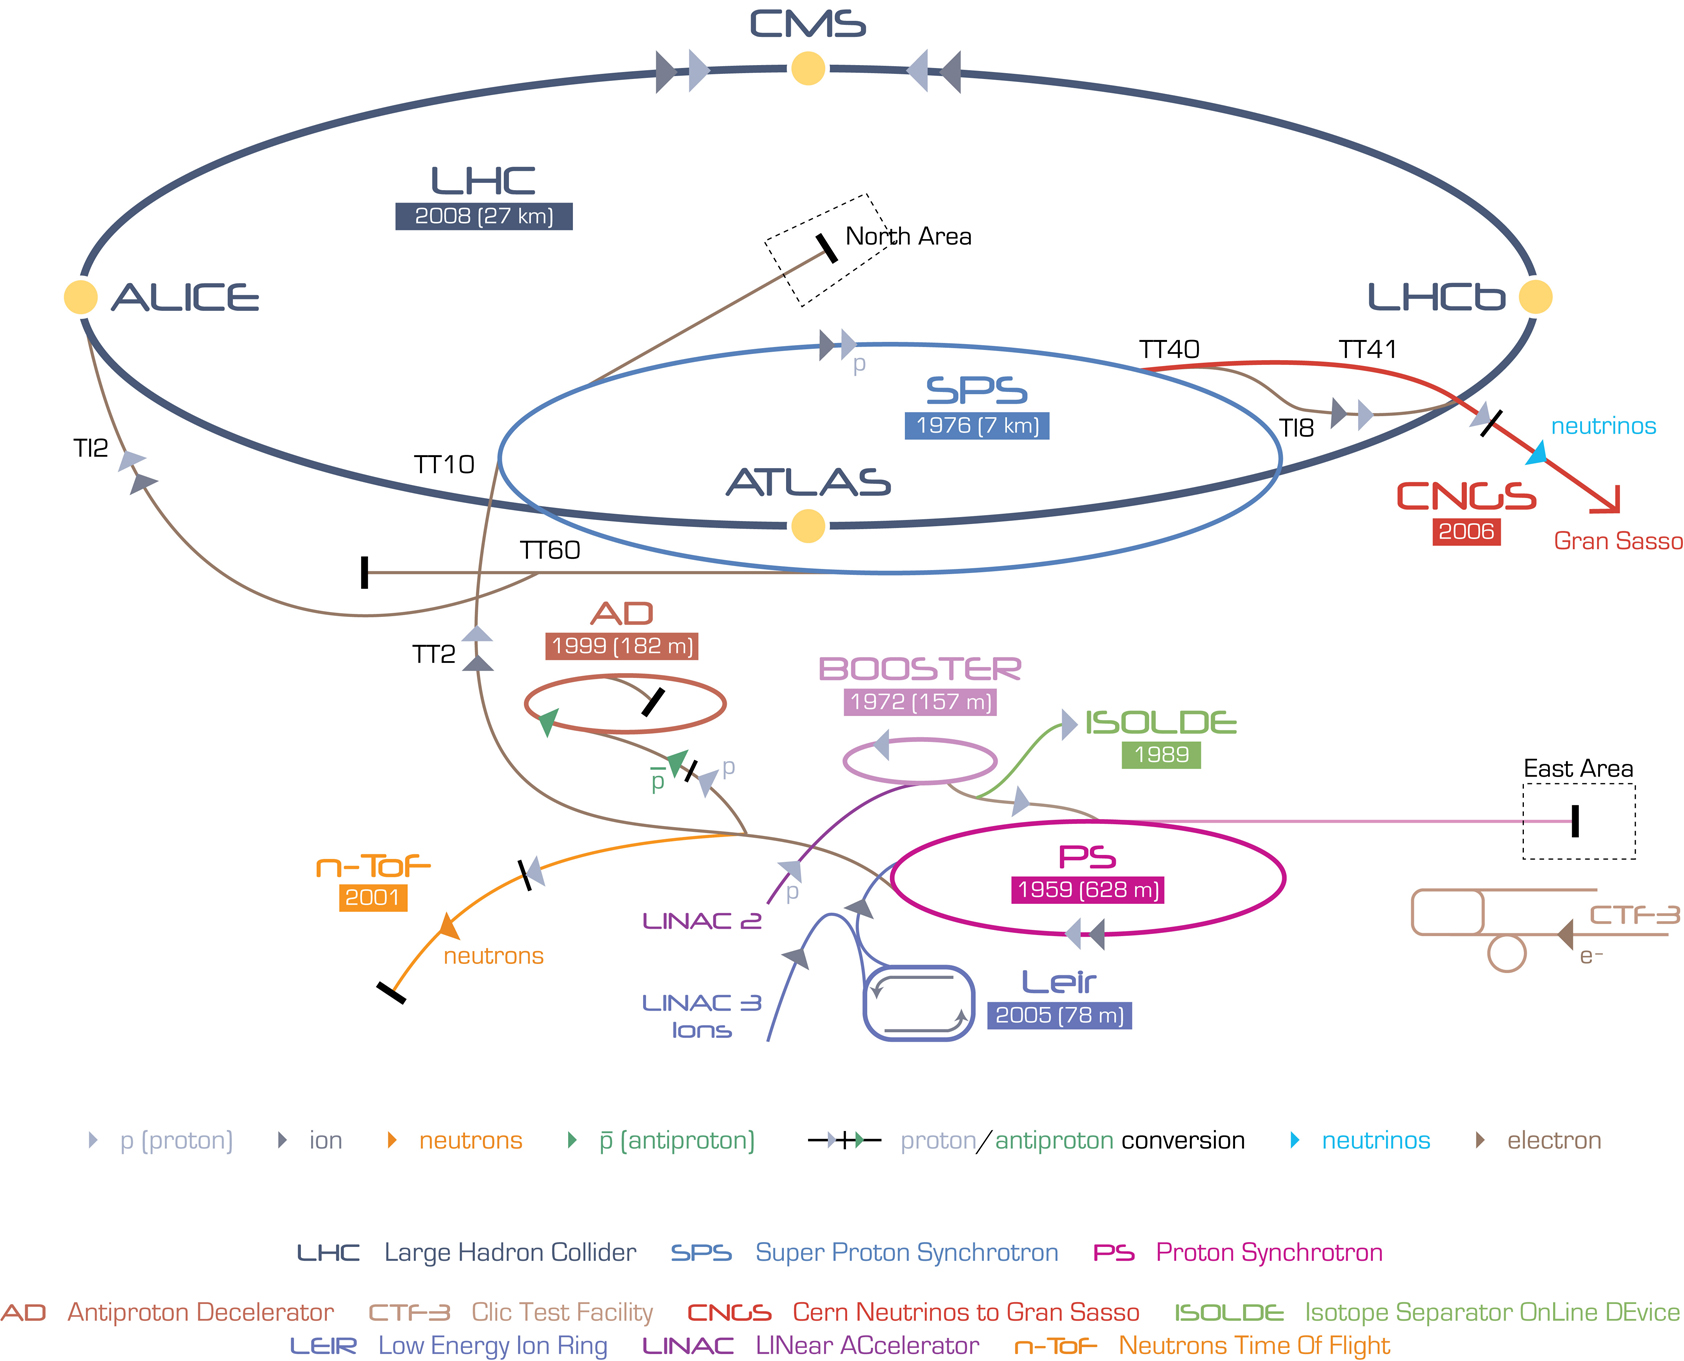
\includegraphics[width=0.8\textwidth]{plots/lhcinjectorchain.jpg}
  \caption{Schematic picture of the injector chain for the LHC~\cite{injchain}.}
  \label{fig:injchain}
\end{figure}

The LHC uses superconducting radio frequency cavities made of niobium to boost the protons to their final energy. Superconducting dipole magnets made of niobium-titanium are used to guide the proton's trajectory. Their $B$-field can reach up to $8\,\text{T}$. Quadrupole, sextupole and octopole magnets are used to clean and focus the beam. The four major experiments are located in caverns, where the two beams are crossing their paths. The ATLAS~\cite{atlasjinst} and CMS~\cite{cmsjinst} experiments are multi-purpose detectors, while ALICE~\cite{alicejinst} is focusing on heavy ions and LHCb~\cite{lhcbjinst} concentrates on b-quark physics.



\section{Compact Muon Solenoid}
\label{sec:cms}

Roughly $100\,\text{m}$ below Cessy (France), at the fifth interaction point (\textbf{IP5}) of the LHC, the Compact Muon Solenoid (\textbf{CMS})~\cite{cmsjinst} is installed (Fig.~\ref{fig:cms}). The cylindrical shape measures $21.6\,\text{m}$ in length and has a diameter of $14.6\,\text{m}$, with an overall weight of $14\,\text{kT}$. It is composed of a large solenoid magnet and a wide variety of sub-detectors, with a \textit{barrel} and an \textit{endcap} region. In combination, they are designed to measure the energy, momentum and trajectory of the particles. The individual components will be discussed in the upcoming sections.

\begin{figure}[ht!]
  \centering
  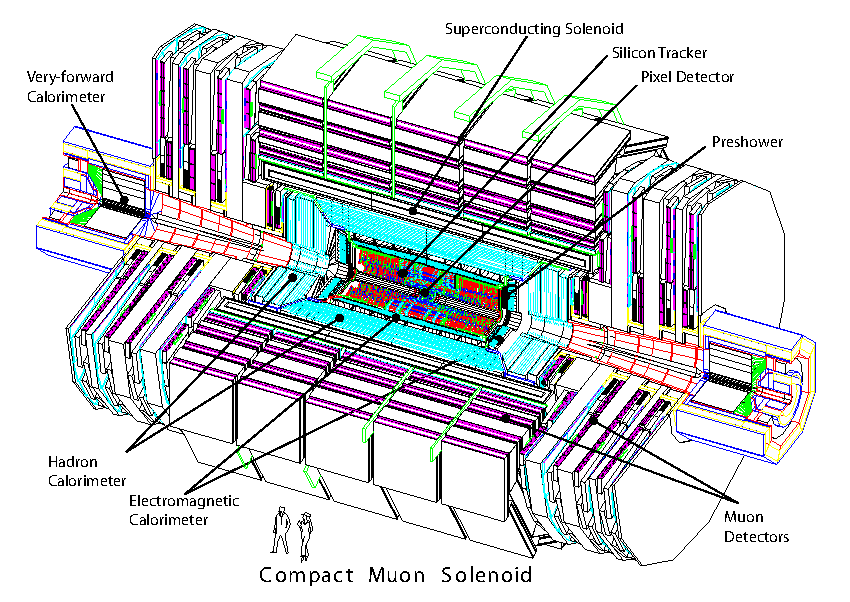
\includegraphics[width=0.8\textwidth]{plots/cms.pdf}
  \caption{Overview of the CMS experiment at the LHC~\cite{cmsjinst}. For a size comparison, two experimentalists are shown.}
  \label{fig:cms}
\end{figure}

The coordinate system chosen by the CMS collaboration places the origin at the nominal collision point of the two proton beams. The $z$-axis is along the path of the proton beams, while the $x$-axis points inward to the center of the LHC ring. That leaves only the vertical, upward direction for the $y$-axis. The radial coordinate $r$ is measured with respect to the nominal interaction point and the azimuth angle $\phi$ is measured in the $x$-$y$ plane. Instead of the polar angle $\theta$, a quantity called ``pseudorapiditiy'' $\eta$ is being used. It is given by $\eta = - \ln{\text{tan}\,\left(\frac{\theta}{2}\right)}$, resulting in differences $\Delta\eta$ being invariant under longitudinal Lorentz boosts. Using the pseudorapidity, the spatial distance between two objects is defined as

\begin{equation}
  \label{eq:spatdiff}
  \Delta R = \sqrt{\left(\Delta \phi\right)^2 + \left(\Delta \eta\right)^2}.
\end{equation}

\subsection{Magnet}

The shape of the magnet is one of the main choices for an experiment. One has to weigh the trajectory bending power against the area density, where the former is essential to measure particle charge and momenta, while the latter can lead to losing or altering particle information due to various effects. The CMS collaboration chose a solenoid shape and thus having a magnetic field parallel to the beam line. One of the distinct features is the superconducting niobium titanium material organized in a 4-layer structure. With the cold mass of the magnet itself being ``only'' $220\,\text{tons}$, the $10\,000\,\text{ton}$ iron yoke surrounding the magnet from the outside is the main contribution to the overall weight. The iron yoke is necessary to return the magnetic flux to the solenoid. With the $3.8\,\text{Tesla}$ the magnet is designed to operate at, it provides excellent bending power in the inner detector. In the muon chambers, only about $2\,\text{T}$ remain.

\subsection{Inner Tracker}
\label{sec:innertracker}

The inner tracker~(Fig.~\ref{fig:inntrk}) is the detector component closest to the collision point. As such, it is faced with the biggest challenges. With about 20 proton-proton collisions up to every $25\,\text{ns}$, not only an extremely fast response time, but also an excellent spatial resolution is necessary. The radiation damage from said interactions also had to be considered. As a result, a detector based on silicon has been chosen and constructed. It has an expect lifetime of 10 years, after which it has to be replaced. The layout of the inner tracker has two components which will be discussed in the next sections.

\begin{figure}[ht!]
  \centering
  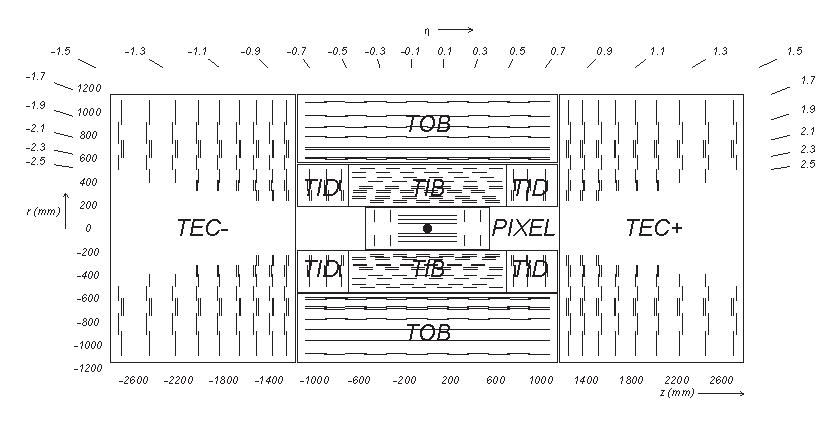
\includegraphics[width=0.8\textwidth]{plots/innertracker.pdf}
  \caption{Layout of the inner tracker of the CMS experiment. Every line represents a silicon detector, whereas the double lines have a secondary micro-strip detector to measure the respective second coordinate~\cite{cmsjinst}.}
  \label{fig:inntrk}
\end{figure}

The \textbf{pixel detector} has its three layers at radii of $4.4$, $7.3$ and $10.2\,\text{cm}$ in the barrel region. Two additional discs are positioned on each side. With an overall amount of $66$ million pixels, it covers an area of roughly $1\,\text{m}^2$. The $100 \times 150\,\mu\text{m}^2$ pixel size provides an excellent track resolution of roughly $15-20\,\mu\text{m}$. This allows for an accurate reconstruction of secondary vertices, giving valuable insight into the decay chains.

Outside of the pixel detector, the \textbf{silicon strip tracker} is extending from $20$ to $116\,\text{cm}$. It has three different subcomponents. The Tracker Inner Barrel (\textbf{TIB}) with its 4 layers and the complementing 3 Tracker Inner Disks (\textbf{TID}) on each side, are positioned parallel and radial to the beam line, respectively. After reaching a radius of $55\,\text{cm}$ the Tracker Outer Barrel (\textbf{TOB}) occupies the remainder of the barrel space with its 6 layers. Following the same structure as the TIB and TID, the endcaps are covered by the Tracker End Caps (\textbf{TEC}), which add another 9 layers of silicon strips. The width and pitch of each strip determine the spatial resolution. It varies between $23$, $35$ and $53\,\mu\text{m}$, with a tendency towards a better resolution the closer the strip is to the collision spot. Additional micro-strip detector modules are attached to the first two layers of the TIB, TID and TOB. Those are used for measuring the second coordinate ($z$ for the barrel region and $r$ in the disks) with a stereo angle of $100\,\text{mrad}$. Overall, the silicon strip tracker has a total of $9.3$ million strips with a surface area of $198\,\text{m}^2$.

Combining both components of the inner tracker, it is possible to measure the transverse momentum of highly energetic tracks ($\sim 100\,\text{GeV}$) with a resolution of $1-2\,\pct$. The geometrical range of $|\eta| < 2.5$ is being covered.


\subsection{Electromagnetic Calorimeter}

As the name suggests, the electromagnetic calorimeter (\textbf{ECAL}) is responsible for measuring electrons and photons. This also includes the electromagnetic component of jets, which is mostly given by $\pi^0 \rightarrow \gamma \gamma$. To simultaneously ensure good response times and a fine granularity\footnote{High density: $8.28\,\text{g/cm}^3$; Short radiation length: $0.89\,\text{cm}$; Small Moli\`{e}re radius: $2.2\,\text{cm}$}, while still being resistant to radiation damage, lead tungstate crystals PbWO$_4$ have been chosen.

The barrel region covered by the calorimeter (\textbf{EB}) spans over $|\eta| < 1.479$. A total of 61200 crystals with a cross section of $22 \times 22\,\text{mm}^2$ near the collision point and $26 \times 26\,\text{mm}^2$ furthest from it, have been mounted. It should be noted that with these dimensions, the Moli\`{e}re radius is able to be contained within a cell, resulting in a good spatial resolution. The length of a cell corresponds to $25.8 X_0$, ensuring the capture of most showers induced by electrons and photons. Avalanche photo diodes (\textbf{APD}) are installed on the outer surface of each cell and are used to measure the scintillation light, which translates to the deposited energy.

In the endcap calorimeters (\textbf{EE}) there are 7324 crystals split into one disk each on both sides. Their coverage extends from $|\eta| < 1.479$ to $|\eta| < 3.0$. However, due to the larger amount of radiation in these directions, the APDs have been replaced by the less efficient, but more resistant vacuum phototriodes (\textbf{VPT}).

To prevent neutral pions from being misidentified as single photons, a preshower detector is installed in front of the crystals in the range of $1.653 < |\eta| < 2.6$. The total thickness of $20\,\text{cm}$ is composed of two layers of lead radiators, which are used to force electromagnetic showering and silicon strip sensors to measure them.

The energy resolution provided by the ECAL for particles below $500\,\text{GeV}$ is given by

\begin{equation}
  \label{eq:ecalreso}
  \left( \frac{ \sigma_E}{E} \right)^2 = \left( \frac{2.8\pct}{\sqrt{E/\text{GeV}}} \right)^2 + \left( \frac{12\pct}{E/\text{GeV}} \right)^2 + (0.3\pct)^2,
\end{equation}

\noindent with the first term being the stochastic contribution, followed by the one from noise and the constant term being added last.


\subsection{Hadronic Calorimeter}

While most electrons and photons can be fully stopped using the ECAL, the nuclear interaction length ($\lambda_I$) of hadrons is much longer, thus allowing them to pass through. The hadronic calorimeter's (\textbf{HCAL}) main priority is the measurement of hadronic jets and other hadronic fragments from proton-proton collisions. The apparent missing transverse energy (\textbf{MET} or $\mathbf{E^{\text{miss}}_{\text{T}}}$) stemming from neutrinos or possibly new particles, can also be estimated by summing up all calorimetric measurements. Overall the HCAL has four sub-components.

The hadron barrel (\textbf{HB}) fills the space between the ECAL ($r = 1.77\,\text{m}$) and the solenoid magnet ($r = 2.95\,\text{m}$) for $|\eta| < 1.3$. It consists of 36 wedges with an individual width of $858\,\text{mm}$. While the top and bottom plate are made of steel, the rest of the absorber material is brass. Depending on the angle $\eta$, one layer of absorber material corresponds to an effective thickness of $5.82$ to $10.6$ interaction lengths $\lambda_I$ (The ECAL provides an additional $1.1\,\lambda_I$). The absorber is followed by plastic scintillators, whose scintillation light is captured by wavelength-shifting fibres and subsequently read out by a hybrid photodiode (\textbf{HPD}).

In the $1.3 < |\eta| < 3.0$ region the hadron endcap (\textbf{HE}) is positioned. It is structured the same way as the HB, with the layers being orthogonal to the beam line, instead of parallel.

Since the HB is very restricted in terms of space, the hadron outer (\textbf{HO}) is added outside of the solenoid magnet. The latter then acts as absorber material. This sub-detector is meant to measure the remainder of hadronic activity, which did not deposit all of its energy in the HB. The wheels in the iron yoke behind the solenoid are equipped with a single layer of HO scintillators, with the exception of the $\eta = 0$ wheel. Due to the absorption material being at its minimum here, an additional $19.5\,\text{cm}$ of iron and a second layer of scintillators is added. Overall the minimal interaction length is increased to $11.8$ in the $|\eta| < 1.3$ region.

The final component, the hadron forward (\textbf{HF}), provides additional coverage for $|\eta| < 5.2$. Due to the exposition to massive amounts of radiation, it is based on grooved steel absorber plates with quartz fibers as an active medium. Although rarely used directly in analyses, the HF provides valuable information for the $E^{\text{miss}}_{\text{T}}$ calculation.

Combining both the ECAL and HCAL, the energy resolution for hadronic showers between $30\,\text{GeV}$ and $1\,\text{TeV}$ is designed to reach~\cite{hcalreso}

\begin{equation}
  \label{eq:hcalreso}
  \left( \frac{\sigma_E}{E} \right)^2 = \left( 100\pct \right)^2 \cdot \frac{\text{GeV}}{E} + (4.5\pct)^2.
\end{equation}


\subsection{Muon System}
\label{sec:muon-system}

One of the central aspects of the CMS experiment, as stated by the second part of the name already, is the detection of muons. With their distinct trajectories muons are very attractive particles to look for. As a result they are part of many signatures, for example the $H \rightarrow ZZ$ decay mode shown in figure~\ref{fig:higgsmzz}. Due to the minimal ionizing nature of muons, most of them pass through the detector, including the calorimeters. This enables one to differentiate between them and other particles, but also implies that it is impossible to measure the energy through deposition in the calorimeters. As a result, the momentum measurement, which depends on the precise track reconstruction, gains that much more importance. This motivates the addition of muon chambers as they can aid in particle identification, provide additional trajectory measurements and can also be used for triggering.

\begin{figure}[!htb]
  \centering
  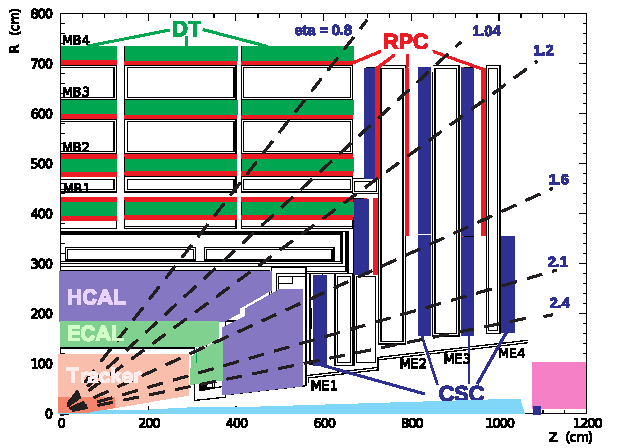
\includegraphics[width=0.8\textwidth]{plots/muonsys.pdf}
  \caption{Cross section of the CMS detector along the beam-pipe~\cite{muonid2}. The regions marked with DT, CSC and RPC represent the muon system components.}
  \label{fig:muonsys}
\end{figure}

The chambers are organized as wheels in the barrel region and disks in the endcap region. The three different types of gas based detectors cover an area of $25\,000\,\text{m}^2$. A wide angle coverage is also ensured by extending up to $|\eta| < 2.4$.

\subsubsection{Drift Tubes}
\label{sec:drift-tubes}

Drift Tubes (\textbf{DT}) are installed in the barrel region ($|\eta| < 1.3$) in between the iron return yoke plates. They operate well with a comparatively low muon rate and a fairly uniform magnetic field, which is contained by the iron yoke. The low cost is also beneficial, considering the large area ($172\,000$ tubes) that needs to be covered in this region. Every drift tube chamber consists of three superlayers, which contain four layers of drift cells. An exemplary cell is shown in figure~\ref{fig:drift-cell}. Overall there are four sets of muon chambers, usually called ``stations''.

\begin{figure}[!htb]
  \centering
  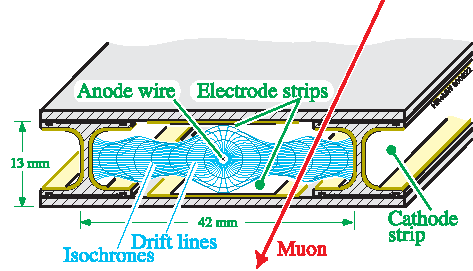
\includegraphics[width=0.5\textwidth]{plots/driftcell.pdf}  
  \caption{Schematic drift cell of the drift tubes in the muon system of the CMS detector~\cite{driftcell}. Both the driftlines and isochrones are shown.}
  \label{fig:drift-cell}
\end{figure}

In the first three stations, the cell in the middle is responsible for measuring the $z$-coordinate, while the other two measure the $r$-$\phi$-component. The fourth station is only equipped with two superlayers, which focus on the $r$-$\phi$ measurement. Each of the $2.4\,\text{m}$ long cells has a gold plated steel wire as an anode in the middle of the chamber with aluminium tape on each side of the wall acting as a cathode. As a muon crosses a cell, it ionizes the argon ($85\pct$), carbon dioxide ($15\pct$) mixture. The resulting electrons (ions) drift towards the anode (cathode), leading to a measurable current. While a single cell has a spatial resolution of $250\,\mu\text{m}$, one station with $2 \times 4$ hits reaches $100,\mu\text{m}$.

\subsubsection{Cathode Strip Chambers}

The endcap region is faced with much higher muon and background fluxes, along with an inhomogeneous magnetic field. As a consequence, cathode strip chambers (\textbf{CSC}) are the detector of choice instead of DTs. They cover the $|\eta|$ range from $0.9$ to $2.4$, overlapping slightly with the DTs. The CSCs are trapezoidally shaped and consist of seven layers of radially oriented cathode strips each. Anode wires are placed perpendicularly to the strips inside the gas filled ($40\pct\,\text{Ar} + 50\pct\,\text{CO}_2 + 10\pct\,\text{CF}_4$) gaps in between each layer. This layout allows for measuring both the $\phi$-component with the strips and the $r$-component with the wires at the same time. The spatial resolution varies between $75\,\mu\text{m}$ and $150\,\mu\text{m}$.

\subsubsection{Resistive Plate Chambers}

The third and final detector type are the resistive plate chambers (\textbf{RPC}). In comparison to the previous two components, they provide much faster response times due to being operated in avalanche mode. In the barrel region, there are overall six RPCs embedded. On the first two drift tube stations, there is one RPC mounted on each side, while only one is installed on each of the two outer stations. Additionally, there are planes of RPCs in between each of the first three stations of the endcap regions. This results in an overall coverage of $|\eta| < 1.6$, which will be expanded in the next upgrade cycle. The detector works with two parallel plates, where the gap is gas filled and read-out strips are placed in the middle. The usage of avalanche mode allows for response times comparable to scintillators, while the geometry yields adequate spatial resolution. \\

By combining the information from both the inner tracker, as well as the muon chambers, an overall transverse momentum resolution of $5\pct$ for highly energetic muons ($\sim 1\,\text{TeV}$) can be reached.



\subsection{Triggering and Data Aquisition}

Upon reaching the design luminosity, there are collisions every $25\,\text{ns}$ corresponding to a rate of proton-proton interactions of about $10^9\,\text{Hz}$. However, the amount of data that is possible to be stored is a few $10^2\,\text{Hz}$. Therefore a preselection, specifically choosing events that potentially contain relevant physics, has to be made. The amount of data to be stored per event is reduced to about $1\,\text{MB}$ in the process. The CMS experiment uses a two-level \textit{trigger} system to perform said reduction.\\

The \textbf{Level-1} (\textbf{L1}) trigger is mostly based upon programmable electronics, which make use of the information provided by the different sub-detectors. Figure~\ref{fig:lvl1trig} shows the information chain of the L1 trigger system. Local triggers collect the basic information from the detector components, which are then combined in regional triggers and are eventually transferred to the global trigger. The latter decides whether or not to discard the event, by performing a preliminary reconstruction. The maximal latency between a bunch crossing and distributing the conclusion to read out the electronics is $3.2\,\mu\text{s}$. Overall, the L1 rate is designed to be about $100\,\text{kHz}$ (typically ran at $98\,\text{kHz}$ during 2012).

If an event is selected by the L1, the front-end buffers of all the sub-detectors are read out and the data is forwarded to the \textbf{data aquisition} (\textbf{DAQ}) system. Here the \textbf{high level trigger} (\textbf{HLT}) performs a much more sophisticated analysis on the collected data. It is able to do so, because it can access all digitized information. This provides an additional reduction to about $2\,\text{kHz}$ (original design rate was $300\,\text{Hz}$).

Distributing the analysed data is the next step. The processed datasets are transferred from the Tier-0 at CERN to the Tier-1 locations, where further analyses are run. Next, it is distributed to the final destination in regards to central storage, the Tier-2 data centers. All CMS workgroups can access the datasets at this stage. It should be noted that the Tier-1 grid is also used for large-scale computing, while the Tier-2 resources are used for analyses.


\begin{figure}[ht!]
  \centering
  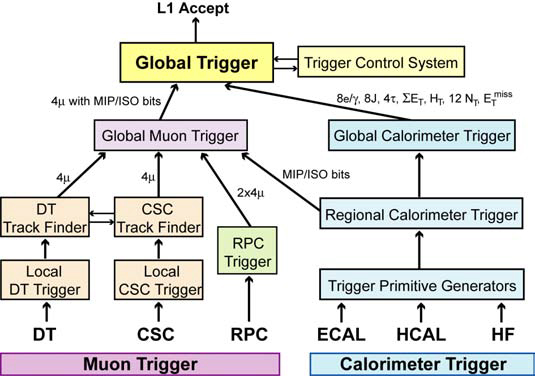
\includegraphics[width=0.55\textwidth]{plots/lvl1trigger.jpg}
  \caption{Schematic overview of the architecture of the Level-1 trigger of the CMS experiment~\cite{cmsjinst}.}
  \label{fig:lvl1trig}
\end{figure}


\subsection{Object Reconstruction}
\label{sec:objreco}

The information provided by the respective sub-detectors, such as a chamber hit or an energy deposit, have to be combined to a physics object for further analysis. Different kinds of objects have individual algorithms. The ones relevant for the analysis will be covered in the next sections. \\

The reconstruction of \textbf{Muons} is solely based on their trajectory. Initially the tracker and muon system hit information are reconstructed separately. If a muon is reconstructed in the muon system, it is considered a \textit{standalone muon}. The Kalman filtering technique~\cite{kalman} is used to reconstruct the trajectory. Starting with a seed, it considers nearby hits to iteratively build the track. Progressing on from the initial standalone muon track, one can compare it to a tracker trajectory by propagating both their parameters to a common plane. If a matching set of hits can be found, the muon becomes a \textit{global muon} which is the most commonly used quantity. Alternatively the initial track can be taken from the tracker. These muon candidate trajectories are then extrapolated by taking various factors like average energy depositions, multiple scattering, precise magnetic field maps and Bremsstrahlung into account. If matching track segments are found in the muon system, the muon becomes a \textit{tracker muon}. The latter is particularly useful for multiple (usually two) collimated muon tracks, as the spatial resolution of the tracker exceeds the one of the muon system by far. \\

\textbf{Jets} are a conglomerate of various, mostly hadronic particles. They usually stem from either a gluon or a quark. As jets are reconstructed as a single object, a specific algorithm has to be chosen to perform this task. A popular choice are sequential recombination algorithms such as the Cambridge/Aachen algorithm. In this analysis the \textbf{anti-$k_\textbf{T}$} clustering algorithm~\cite{antikt} will be used. It is both collinear and infrared safe, meaning that the reconstruction is neither significantly affected by splitting in the collinear direction nor the emission of soft particles. Unlike the other sequential recombination algorithms, this method provides a conical shape for which the cone radius parameter will be set to $R = 0.5$.

Both \textbf{electrons} and \textbf{photons} are mainly measured via the ECAL~\cite{elereco}. While the electron radiates photons as its trajectory is bent by the magnetic field, photons with sufficient energy can lead to pair production under the influence of electromagnetic fields. In combination, this leads to an electromagnetic shower, which covers a cluster of roughly $5 \times 5$ ECAL cells for particles of intermediate energies. Measuring this shower allows for estimation of the energy of the initial particle. An additional transverse momentum measurement from the tracker is also possible for tracks of charged particles. Building these is initiated by superclusters (clusters of clusters) in the pixel detector and uses a Gaussian Sum Filter with a specific energy loss model.

While photons do not carry any charge, they tend to produce electron-positron pairs when under the influence of an atom's electric field. Electrons also radiate photons as they are subject to the Coulomb field of a nucleus, which are then again able to lead to pair production. As such, both types of objects produce a particle track until their energy has decreased sufficiently that they can be absorbed into the detector material.

\textbf{Missing transverse energy} is calculated from the vectorial sum of the transverse energies of all reconstructed objects. As one expects the initial state of a proton-proton collision to only have a negligible amount of transverse energy, the aforementioned sum should be zero. However, certain particles such as neutrinos or possibly new, yet unknown ones can escape the detector. The negative value of the vectorial sum is the collective estimate for all particles that avoided detection.

While most reconstruction algorithms work independently from one another to identify particle candidates, the \textbf{particle-flow} algorithm~\cite{pflow} reconstructs entire events. This means, that the tracks of every muon, electron, photon, as well as the charged and neutral hadrons are being taken into account when identifying particles. Consequently it is necessary to consider all sub-detectors and the information they provide. Overall, the expected performance for accurately identifying and reconstructing jets, taus and missing transverse energy is improved. Taking jets as an example, the components each jet consists of are reconstructed individually. Instead of approximating the shape through a cone, even the low energy fragments with diverging tracks can be assigned to the right jets. Taking all the information (that the algorithm considers) about nearby particles into account, an in-depth isolation criterion can be defined. This is particularly useful for muons used in this analysis.



%%% Local Variables: 
%%% mode: latex
%%% TeX-master: "document"
%%% End: 
